
\begin{figure*}[t]
    \centering
    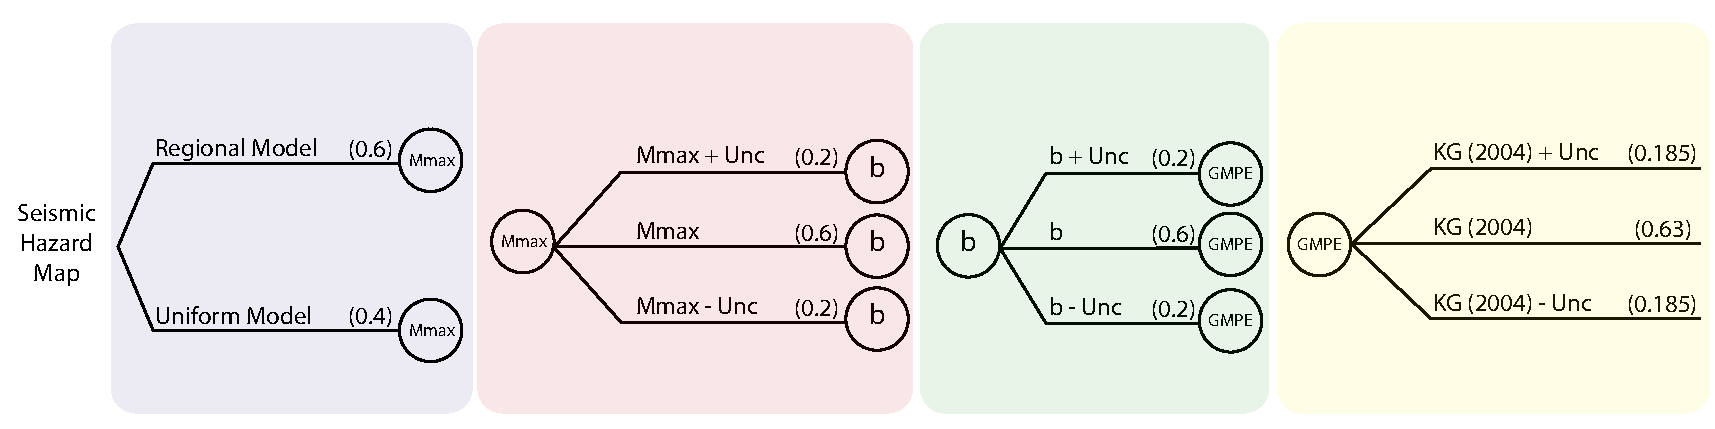
\includegraphics[width=\textwidth]{figures/pdf/figure-09}
    \caption{Logic tree nodes and associated weights used in the seismic hazard analysis for northern Iran.}
    \label{fig:logic}
\end{figure*}

\section{\myrevision{Logic Tree}}

\myrevision{As mentioned in previous sections, we address the uncertainties in our models, seismic parameters and selected ground motion prediction equation via a logic tree. Fig.~\ref{fig:logic} shows the complete set of branches at each of the tree nodes. In particular, we consider uncertainty in the seismic zonation via the combination of the R and U models, the maximum magnitude $M_{\max}$, the seismic $b$-value, and the prediction of PGA intensities in the GMPE by \citet{Kalkan2004}. We assigned the weights to the R and U model arbitrarily, giving more weight to the regional model R based on the expectation that a regionalized model would likely lead to a better seismic hazard analysis. Other weights in the logic tree are based on previous studies \citep[e.g.,][]{Petersen2015}.}

\myrevision{Among other possible parameters for which we could have consider additional sources of uncertainty, we note that we did not consider the variability of the reference depth and seismic velocities in the selected GMPE because these were values fixed to satisfy the fit of the equation with data from northern Iran. Thus introducing uncertainty in these parameters would have been to the detriment of the prediction of PGA values.}

 % We considered the uncertainty in tectonic seismic region through adding the uniform model with lower weight than the most recent accepted classification.}
